\documentclass{whiteboard}
\begin{document}
\begin{frame}[plain,t]
\bbcover{CSES 1202}{Investigation}{Prof. Edson Alves}{Faculdade UnB Gama}

\end{frame}
\begin{frame}[plain,t]
\vspace*{\fill}

\bbenglish{You are going to travel from Syrjälä to Lehmälä by plane. You would like to find answers to the following questions:}

\vspace{0.2in}

\begin{itemize}
\item \bbenglish{what is the minimum price of such a route?}
\item \bbenglish{how many minimum-price routes are there? (modulo $10^9+7$)}
\item \bbenglish{what is the minimum number of flights in a minimum-price route?}
\item \bbenglish{what is the maximum number of flights in a minimum-price route?}
\end{itemize}

\vspace*{\fill}
\end{frame}
\begin{frame}[plain,t]
\vspace*{\fill}

\bbtext{Você irá viajar de Syrjälä para Lehmälä de avião. Você gostaria de encontrar respostas para as seguintes questões:}

\vspace{0.2in}

\begin{itemize}
\item \bbtext{qual é o preço mínimo de tal rota?}
\item \bbtext{existem quantas rotas de preço mínimo? (módulo $10^9+7$)}
\item \bbtext{qual é o número mínimo de voôs em uma rota de preço mínimo?}
\item \bbtext{qual é o número máximo de voôs em uma rota de preço mínimo?}
\end{itemize}

\vspace*{\fill}
\end{frame}
\begin{frame}[plain,t]
\vspace*{\fill}

\bbbold{Input}

\vspace{0.1in}

\bbenglish{The first input line contains two integers $n$ and $m$: the number of cities and the number of flights. The cities are numbered $1, 2, \ldots, n$. City $1$ is Syrjälä, and city $n$ is Lehmälä.}

\vspace{0.1in}

\bbenglish{After this, there are $m$ lines describing the flights. Each line has three integers $a, b,$ and $c$: there is a flight from city $a$ to city $b$ with price $c$. All flights are one-way flights.}

\vspace{0.1in}

\bbenglish{You may assume that there is a route from Syrjälä to Lehmälä.}

\vspace*{\fill}
\end{frame}
\begin{frame}[plain,t]
\vspace*{\fill}

\bbbold{Entrada}

\vspace{0.1in}

\bbtext{A primeira linha da entrada contém dois inteiros $n$ e $m$: o número de cidades e o número de vôos. As cidades são numeradas $1, 2, \ldots, n$. A cidade $1$ é Syrjälä e a cidade $n$ é Lehmälä.}

\vspace{0.1in}

\bbtext{Após isto, há $m$ linhas descrevendo os vôos. Cada linha tem três inteiros $a, b,$ e $c$: há um vôo da cidade $a$ para a cidade $b$ com preço $c$. Todos vôos são dados em sentido único.}

\vspace{0.1in}

\bbtext{Você pode assumir que existe uma rota de Syrjälä para Lehmälä.}

\vspace*{\fill}
\end{frame}
\begin{frame}[plain,t]
\vspace*{\fill}

\bbbold{Output}

\vspace{0.1in}

\bbenglish{Print four integers according to the problem statement.}

\vspace{0.2in}

\bbbold{Constraints}

\vspace{0.1in}

\begin{itemize}
\item $1\leq n\leq 10^5$
\item $1\leq m\leq 2\times 10^5$
\item $1\leq a, b\leq n$
\item $1\leq c\leq 10^9$
\end{itemize}

\vspace*{\fill}
\end{frame}
\begin{frame}[plain,t]
\vspace*{\fill}

\bbbold{Saída}

\vspace{0.1in}

\bbtext{Imprima quatro inteiros, de acordo com o texto do problema.}

\vspace{0.2in}

\bbbold{Restrições}

\vspace{0.1in}

\begin{itemize}
\item $1\leq n\leq 10^5$
\item $1\leq m\leq 2\times 10^5$
\item $1\leq a, b\leq n$
\item $1\leq c\leq 10^9$
\end{itemize}

\vspace*{\fill}
\end{frame}
\begin{frame}[plain,t]
\begin{tikzpicture}
\node[draw,opacity=0] at (0, 0) {x};
\node[draw,opacity=0] at (14, 8) {x};

	\node[anchor=west] (header) at (0, 7.0) { \bbbold{Exemplo de entrada e saída} };

\end{tikzpicture}
\end{frame}
\begin{frame}[plain,t]
\begin{tikzpicture}
\node[draw,opacity=0] at (0, 0) {x};
\node[draw,opacity=0] at (14, 8) {x};

	\node[anchor=west] (header) at (0, 7.0) { \bbbold{Exemplo de entrada e saída} };


	\node[anchor=west] (line1) at (1.0, 6.0) { \bbtext{\texttt{4 5} } };

\end{tikzpicture}
\end{frame}
\begin{frame}[plain,t]
\begin{tikzpicture}
\node[draw,opacity=0] at (0, 0) {x};
\node[draw,opacity=0] at (14, 8) {x};

	\node[anchor=west] (header) at (0, 7.0) { \bbbold{Exemplo de entrada e saída} };


	\node[anchor=west] (line1) at (1.0, 6.0) { \bbtext{\texttt{4 5} } };


	\draw[->,color=BBViolet] (1.25, 5.0) to  (1.25, 5.75);

	\node[] (r) at (1.25, 4.75) { \footnotesize \bbcomment{\# de cidades} };

\end{tikzpicture}
\end{frame}
\begin{frame}[plain,t]
\begin{tikzpicture}
\node[draw,opacity=0] at (0, 0) {x};
\node[draw,opacity=0] at (14, 8) {x};

	\node[anchor=west] (header) at (0, 7.0) { \bbbold{Exemplo de entrada e saída} };


	\node[anchor=west] (line1) at (1.0, 6.0) { \bbtext{\texttt{4 5} } };


	\draw[->,color=BBViolet] (1.65, 5.0) to  (1.65, 5.75);

	\node[] (r) at (1.65, 4.75) { \footnotesize \bbcomment{\# de vôos} };



\end{tikzpicture}
\end{frame}
\begin{frame}[plain,t]
\begin{tikzpicture}
\node[draw,opacity=0] at (0, 0) {x};
\node[draw,opacity=0] at (14, 8) {x};

	\node[anchor=west] (header) at (0, 7.0) { \bbbold{Exemplo de entrada e saída} };


	\node[anchor=west] (line1) at (1.0, 6.0) { \bbtext{\texttt{4 5} } };







	\node[draw,very thick,circle] (node1) at (7.0, 4.0) { \bbtext{1} };

	\node[draw,very thick,circle] (node2) at (10.0, 7.0) { \bbtext{2} };

	\node[draw,very thick,circle] (node3) at (13.0, 4.0) { \bbtext{3} };

	\node[draw,very thick,circle] (node4) at (10.0, 1.0) { \bbtext{4} };

\end{tikzpicture}
\end{frame}
\begin{frame}[plain,t]
\begin{tikzpicture}
\node[draw,opacity=0] at (0, 0) {x};
\node[draw,opacity=0] at (14, 8) {x};

	\node[anchor=west] (header) at (0, 7.0) { \bbbold{Exemplo de entrada e saída} };


	\node[anchor=west] (line1) at (1.0, 6.0) { \bbtext{\texttt{4 5} } };







	\node[draw,very thick,circle] (node1) at (7.0, 4.0) { \bbtext{1} };

	\node[draw,very thick,circle] (node2) at (10.0, 7.0) { \bbtext{2} };

	\node[draw,very thick,circle] (node3) at (13.0, 4.0) { \bbtext{3} };

	\node[draw,very thick,circle] (node4) at (10.0, 1.0) { \bbtext{4} };


	\node[anchor=west] (line2) at (1.0, 5.5) { \bbtext{\texttt{1 4 5}} };

\end{tikzpicture}
\end{frame}
\begin{frame}[plain,t]
\begin{tikzpicture}
\node[draw,opacity=0] at (0, 0) {x};
\node[draw,opacity=0] at (14, 8) {x};

	\node[anchor=west] (header) at (0, 7.0) { \bbbold{Exemplo de entrada e saída} };


	\node[anchor=west] (line1) at (1.0, 6.0) { \bbtext{\texttt{4 5} } };


	\draw[->,color=BBViolet] (1.25, 4.25) to  (1.25, 5.25);

	\node[] (r) at (1.25, 4.0) { \footnotesize \bbcomment{$a$} };




	\node[draw,very thick,circle] (node1) at (7.0, 4.0) { \bbtext{1} };

	\node[draw,very thick,circle] (node2) at (10.0, 7.0) { \bbtext{2} };

	\node[draw,very thick,circle] (node3) at (13.0, 4.0) { \bbtext{3} };

	\node[draw,very thick,circle] (node4) at (10.0, 1.0) { \bbtext{4} };


	\node[anchor=west] (line2) at (1.0, 5.5) { \bbtext{\texttt{1 4 5}} };



\end{tikzpicture}
\end{frame}
\begin{frame}[plain,t]
\begin{tikzpicture}
\node[draw,opacity=0] at (0, 0) {x};
\node[draw,opacity=0] at (14, 8) {x};

	\node[anchor=west] (header) at (0, 7.0) { \bbbold{Exemplo de entrada e saída} };


	\node[anchor=west] (line1) at (1.0, 6.0) { \bbtext{\texttt{4 5} } };


	\draw[->,color=BBViolet] (1.65, 4.25) to  (1.65, 5.25);

	\node[] (r) at (1.65, 4.0) { \footnotesize \bbcomment{$b$} };




	\node[draw,very thick,circle] (node1) at (7.0, 4.0) { \bbtext{1} };

	\node[draw,very thick,circle] (node2) at (10.0, 7.0) { \bbtext{2} };

	\node[draw,very thick,circle] (node3) at (13.0, 4.0) { \bbtext{3} };

	\node[draw,very thick,circle] (node4) at (10.0, 1.0) { \bbtext{4} };


	\node[anchor=west] (line2) at (1.0, 5.5) { \bbtext{\texttt{1 4 5}} };






\end{tikzpicture}
\end{frame}
\begin{frame}[plain,t]
\begin{tikzpicture}
\node[draw,opacity=0] at (0, 0) {x};
\node[draw,opacity=0] at (14, 8) {x};

	\node[anchor=west] (header) at (0, 7.0) { \bbbold{Exemplo de entrada e saída} };


	\node[anchor=west] (line1) at (1.0, 6.0) { \bbtext{\texttt{4 5} } };


	\draw[->,color=BBViolet] (2.05, 4.25) to  (2.05, 5.25);

	\node[] (r) at (2.05, 4.0) { \footnotesize \bbcomment{$c$} };




	\node[draw,very thick,circle] (node1) at (7.0, 4.0) { \bbtext{1} };

	\node[draw,very thick,circle] (node2) at (10.0, 7.0) { \bbtext{2} };

	\node[draw,very thick,circle] (node3) at (13.0, 4.0) { \bbtext{3} };

	\node[draw,very thick,circle] (node4) at (10.0, 1.0) { \bbtext{4} };


	\node[anchor=west] (line2) at (1.0, 5.5) { \bbtext{\texttt{1 4 5}} };









\end{tikzpicture}
\end{frame}
\begin{frame}[plain,t]
\begin{tikzpicture}
\node[draw,opacity=0] at (0, 0) {x};
\node[draw,opacity=0] at (14, 8) {x};

	\node[anchor=west] (header) at (0, 7.0) { \bbbold{Exemplo de entrada e saída} };


	\node[anchor=west] (line1) at (1.0, 6.0) { \bbtext{\texttt{4 5} } };







	\node[draw,very thick,circle] (node1) at (7.0, 4.0) { \bbtext{1} };

	\node[draw,very thick,circle] (node2) at (10.0, 7.0) { \bbtext{2} };

	\node[draw,very thick,circle] (node3) at (13.0, 4.0) { \bbtext{3} };

	\node[draw,very thick,circle] (node4) at (10.0, 1.0) { \bbtext{4} };


	\node[anchor=west] (line2) at (1.0, 5.5) { \bbtext{\texttt{1 4 5}} };










	\draw[thick,-latex](node1) to node[below left] { \bbinfo{5} } (node4);

\end{tikzpicture}
\end{frame}
\begin{frame}[plain,t]
\begin{tikzpicture}
\node[draw,opacity=0] at (0, 0) {x};
\node[draw,opacity=0] at (14, 8) {x};

	\node[anchor=west] (header) at (0, 7.0) { \bbbold{Exemplo de entrada e saída} };


	\node[anchor=west] (line1) at (1.0, 6.0) { \bbtext{\texttt{4 5} } };







	\node[draw,very thick,circle] (node1) at (7.0, 4.0) { \bbtext{1} };

	\node[draw,very thick,circle] (node2) at (10.0, 7.0) { \bbtext{2} };

	\node[draw,very thick,circle] (node3) at (13.0, 4.0) { \bbtext{3} };

	\node[draw,very thick,circle] (node4) at (10.0, 1.0) { \bbtext{4} };


	\node[anchor=west] (line2) at (1.0, 5.5) { \bbtext{\texttt{1 4 5}} };










	\draw[thick,-latex](node1) to node[below left] { \bbinfo{5} } (node4);


	\node[anchor=west] (line3) at (1.0, 5.0) { \bbtext{\texttt{1 2 4} } };

\end{tikzpicture}
\end{frame}
\begin{frame}[plain,t]
\begin{tikzpicture}
\node[draw,opacity=0] at (0, 0) {x};
\node[draw,opacity=0] at (14, 8) {x};

	\node[anchor=west] (header) at (0, 7.0) { \bbbold{Exemplo de entrada e saída} };


	\node[anchor=west] (line1) at (1.0, 6.0) { \bbtext{\texttt{4 5} } };







	\node[draw,very thick,circle] (node1) at (7.0, 4.0) { \bbtext{1} };

	\node[draw,very thick,circle] (node2) at (10.0, 7.0) { \bbtext{2} };

	\node[draw,very thick,circle] (node3) at (13.0, 4.0) { \bbtext{3} };

	\node[draw,very thick,circle] (node4) at (10.0, 1.0) { \bbtext{4} };


	\node[anchor=west] (line2) at (1.0, 5.5) { \bbtext{\texttt{1 4 5}} };










	\draw[thick,-latex](node1) to node[below left] { \bbinfo{5} } (node4);


	\node[anchor=west] (line3) at (1.0, 5.0) { \bbtext{\texttt{1 2 4} } };

	\draw[thick,-latex](node1) to node[above left] { \bbinfo{4} } (node2);

\end{tikzpicture}
\end{frame}
\begin{frame}[plain,t]
\begin{tikzpicture}
\node[draw,opacity=0] at (0, 0) {x};
\node[draw,opacity=0] at (14, 8) {x};

	\node[anchor=west] (header) at (0, 7.0) { \bbbold{Exemplo de entrada e saída} };


	\node[anchor=west] (line1) at (1.0, 6.0) { \bbtext{\texttt{4 5} } };







	\node[draw,very thick,circle] (node1) at (7.0, 4.0) { \bbtext{1} };

	\node[draw,very thick,circle] (node2) at (10.0, 7.0) { \bbtext{2} };

	\node[draw,very thick,circle] (node3) at (13.0, 4.0) { \bbtext{3} };

	\node[draw,very thick,circle] (node4) at (10.0, 1.0) { \bbtext{4} };


	\node[anchor=west] (line2) at (1.0, 5.5) { \bbtext{\texttt{1 4 5}} };










	\draw[thick,-latex](node1) to node[below left] { \bbinfo{5} } (node4);


	\node[anchor=west] (line3) at (1.0, 5.0) { \bbtext{\texttt{1 2 4} } };

	\draw[thick,-latex](node1) to node[above left] { \bbinfo{4} } (node2);


	\node[anchor=west] (line4) at (1.0, 4.5) { \bbtext{\texttt{2 4 5} } };

\end{tikzpicture}
\end{frame}
\begin{frame}[plain,t]
\begin{tikzpicture}
\node[draw,opacity=0] at (0, 0) {x};
\node[draw,opacity=0] at (14, 8) {x};

	\node[anchor=west] (header) at (0, 7.0) { \bbbold{Exemplo de entrada e saída} };


	\node[anchor=west] (line1) at (1.0, 6.0) { \bbtext{\texttt{4 5} } };







	\node[draw,very thick,circle] (node1) at (7.0, 4.0) { \bbtext{1} };

	\node[draw,very thick,circle] (node2) at (10.0, 7.0) { \bbtext{2} };

	\node[draw,very thick,circle] (node3) at (13.0, 4.0) { \bbtext{3} };

	\node[draw,very thick,circle] (node4) at (10.0, 1.0) { \bbtext{4} };


	\node[anchor=west] (line2) at (1.0, 5.5) { \bbtext{\texttt{1 4 5}} };










	\draw[thick,-latex](node1) to node[below left] { \bbinfo{5} } (node4);


	\node[anchor=west] (line3) at (1.0, 5.0) { \bbtext{\texttt{1 2 4} } };

	\draw[thick,-latex](node1) to node[above left] { \bbinfo{4} } (node2);


	\node[anchor=west] (line4) at (1.0, 4.5) { \bbtext{\texttt{2 4 5} } };

	\draw[thick,-latex](node2) to node[left, pos=0.7] { \bbinfo{5} } (node4);

\end{tikzpicture}
\end{frame}
\begin{frame}[plain,t]
\begin{tikzpicture}
\node[draw,opacity=0] at (0, 0) {x};
\node[draw,opacity=0] at (14, 8) {x};

	\node[anchor=west] (header) at (0, 7.0) { \bbbold{Exemplo de entrada e saída} };


	\node[anchor=west] (line1) at (1.0, 6.0) { \bbtext{\texttt{4 5} } };







	\node[draw,very thick,circle] (node1) at (7.0, 4.0) { \bbtext{1} };

	\node[draw,very thick,circle] (node2) at (10.0, 7.0) { \bbtext{2} };

	\node[draw,very thick,circle] (node3) at (13.0, 4.0) { \bbtext{3} };

	\node[draw,very thick,circle] (node4) at (10.0, 1.0) { \bbtext{4} };


	\node[anchor=west] (line2) at (1.0, 5.5) { \bbtext{\texttt{1 4 5}} };










	\draw[thick,-latex](node1) to node[below left] { \bbinfo{5} } (node4);


	\node[anchor=west] (line3) at (1.0, 5.0) { \bbtext{\texttt{1 2 4} } };

	\draw[thick,-latex](node1) to node[above left] { \bbinfo{4} } (node2);


	\node[anchor=west] (line4) at (1.0, 4.5) { \bbtext{\texttt{2 4 5} } };

	\draw[thick,-latex](node2) to node[left, pos=0.7] { \bbinfo{5} } (node4);


	\node[anchor=west] (line5) at (1.0, 4.0) { \bbtext{\texttt{1 3 2} } };

\end{tikzpicture}
\end{frame}
\begin{frame}[plain,t]
\begin{tikzpicture}
\node[draw,opacity=0] at (0, 0) {x};
\node[draw,opacity=0] at (14, 8) {x};

	\node[anchor=west] (header) at (0, 7.0) { \bbbold{Exemplo de entrada e saída} };


	\node[anchor=west] (line1) at (1.0, 6.0) { \bbtext{\texttt{4 5} } };







	\node[draw,very thick,circle] (node1) at (7.0, 4.0) { \bbtext{1} };

	\node[draw,very thick,circle] (node2) at (10.0, 7.0) { \bbtext{2} };

	\node[draw,very thick,circle] (node3) at (13.0, 4.0) { \bbtext{3} };

	\node[draw,very thick,circle] (node4) at (10.0, 1.0) { \bbtext{4} };


	\node[anchor=west] (line2) at (1.0, 5.5) { \bbtext{\texttt{1 4 5}} };










	\draw[thick,-latex](node1) to node[below left] { \bbinfo{5} } (node4);


	\node[anchor=west] (line3) at (1.0, 5.0) { \bbtext{\texttt{1 2 4} } };

	\draw[thick,-latex](node1) to node[above left] { \bbinfo{4} } (node2);


	\node[anchor=west] (line4) at (1.0, 4.5) { \bbtext{\texttt{2 4 5} } };

	\draw[thick,-latex](node2) to node[left, pos=0.7] { \bbinfo{5} } (node4);


	\node[anchor=west] (line5) at (1.0, 4.0) { \bbtext{\texttt{1 3 2} } };

	\draw[thick,-latex](node1) to node[above,pos=0.7] { \bbinfo{2} } (node3);

\end{tikzpicture}
\end{frame}
\begin{frame}[plain,t]
\begin{tikzpicture}
\node[draw,opacity=0] at (0, 0) {x};
\node[draw,opacity=0] at (14, 8) {x};

	\node[anchor=west] (header) at (0, 7.0) { \bbbold{Exemplo de entrada e saída} };


	\node[anchor=west] (line1) at (1.0, 6.0) { \bbtext{\texttt{4 5} } };







	\node[draw,very thick,circle] (node1) at (7.0, 4.0) { \bbtext{1} };

	\node[draw,very thick,circle] (node2) at (10.0, 7.0) { \bbtext{2} };

	\node[draw,very thick,circle] (node3) at (13.0, 4.0) { \bbtext{3} };

	\node[draw,very thick,circle] (node4) at (10.0, 1.0) { \bbtext{4} };


	\node[anchor=west] (line2) at (1.0, 5.5) { \bbtext{\texttt{1 4 5}} };










	\draw[thick,-latex](node1) to node[below left] { \bbinfo{5} } (node4);


	\node[anchor=west] (line3) at (1.0, 5.0) { \bbtext{\texttt{1 2 4} } };

	\draw[thick,-latex](node1) to node[above left] { \bbinfo{4} } (node2);


	\node[anchor=west] (line4) at (1.0, 4.5) { \bbtext{\texttt{2 4 5} } };

	\draw[thick,-latex](node2) to node[left, pos=0.7] { \bbinfo{5} } (node4);


	\node[anchor=west] (line5) at (1.0, 4.0) { \bbtext{\texttt{1 3 2} } };

	\draw[thick,-latex](node1) to node[above,pos=0.7] { \bbinfo{2} } (node3);


	\node[anchor=west] (line6) at (1.0, 3.5) { \bbtext{\texttt{3 4 3} } };

\end{tikzpicture}
\end{frame}
\begin{frame}[plain,t]
\begin{tikzpicture}
\node[draw,opacity=0] at (0, 0) {x};
\node[draw,opacity=0] at (14, 8) {x};

	\node[anchor=west] (header) at (0, 7.0) { \bbbold{Exemplo de entrada e saída} };


	\node[anchor=west] (line1) at (1.0, 6.0) { \bbtext{\texttt{4 5} } };







	\node[draw,very thick,circle] (node1) at (7.0, 4.0) { \bbtext{1} };

	\node[draw,very thick,circle] (node2) at (10.0, 7.0) { \bbtext{2} };

	\node[draw,very thick,circle] (node3) at (13.0, 4.0) { \bbtext{3} };

	\node[draw,very thick,circle] (node4) at (10.0, 1.0) { \bbtext{4} };


	\node[anchor=west] (line2) at (1.0, 5.5) { \bbtext{\texttt{1 4 5}} };










	\draw[thick,-latex](node1) to node[below left] { \bbinfo{5} } (node4);


	\node[anchor=west] (line3) at (1.0, 5.0) { \bbtext{\texttt{1 2 4} } };

	\draw[thick,-latex](node1) to node[above left] { \bbinfo{4} } (node2);


	\node[anchor=west] (line4) at (1.0, 4.5) { \bbtext{\texttt{2 4 5} } };

	\draw[thick,-latex](node2) to node[left, pos=0.7] { \bbinfo{5} } (node4);


	\node[anchor=west] (line5) at (1.0, 4.0) { \bbtext{\texttt{1 3 2} } };

	\draw[thick,-latex](node1) to node[above,pos=0.7] { \bbinfo{2} } (node3);


	\node[anchor=west] (line6) at (1.0, 3.5) { \bbtext{\texttt{3 4 3} } };

	\draw[thick,-latex](node3) to node[below right] { \bbinfo{3} } (node4);

\end{tikzpicture}
\end{frame}
\begin{frame}[plain,t]
\begin{tikzpicture}
\node[draw,opacity=0] at (0, 0) {x};
\node[draw,opacity=0] at (14, 8) {x};

	\node[anchor=west] (header) at (0, 7.0) { \bbbold{Exemplo de entrada e saída} };


	\node[anchor=west] (line1) at (1.0, 6.0) { \bbtext{\texttt{4 5} } };







	\node[draw,very thick,circle,fill=BBGreen] (node1) at (7.0, 4.0) { \bbtext{1} };

	\node[draw,very thick,circle] (node2) at (10.0, 7.0) { \bbtext{2} };

	\node[draw,very thick,circle] (node3) at (13.0, 4.0) { \bbtext{3} };

	\node[draw,very thick,circle] (node4) at (10.0, 1.0) { \bbtext{4} };


	\node[anchor=west] (line2) at (1.0, 5.5) { \bbtext{\texttt{1 4 5}} };










	\draw[thick,-latex](node1) to node[below left] { \bbinfo{5} } (node4);


	\node[anchor=west] (line3) at (1.0, 5.0) { \bbtext{\texttt{1 2 4} } };

	\draw[thick,-latex](node1) to node[above left] { \bbinfo{4} } (node2);


	\node[anchor=west] (line4) at (1.0, 4.5) { \bbtext{\texttt{2 4 5} } };

	\draw[thick,-latex](node2) to node[left, pos=0.7] { \bbinfo{5} } (node4);


	\node[anchor=west] (line5) at (1.0, 4.0) { \bbtext{\texttt{1 3 2} } };

	\draw[thick,-latex](node1) to node[above,pos=0.7] { \bbinfo{2} } (node3);


	\node[anchor=west] (line6) at (1.0, 3.5) { \bbtext{\texttt{3 4 3} } };

	\draw[thick,-latex](node3) to node[below right] { \bbinfo{3} } (node4);


\end{tikzpicture}
\end{frame}
\begin{frame}[plain,t]
\begin{tikzpicture}
\node[draw,opacity=0] at (0, 0) {x};
\node[draw,opacity=0] at (14, 8) {x};

	\node[anchor=west] (header) at (0, 7.0) { \bbbold{Exemplo de entrada e saída} };


	\node[anchor=west] (line1) at (1.0, 6.0) { \bbtext{\texttt{4 5} } };







	\node[draw,very thick,circle,fill=BBGreen] (node1) at (7.0, 4.0) { \bbtext{1} };

	\node[draw,very thick,circle] (node2) at (10.0, 7.0) { \bbtext{2} };

	\node[draw,very thick,circle] (node3) at (13.0, 4.0) { \bbtext{3} };

	\node[draw,very thick,circle,fill=BBCyan] (node4) at (10.0, 1.0) { \bbtext{4} };


	\node[anchor=west] (line2) at (1.0, 5.5) { \bbtext{\texttt{1 4 5}} };










	\draw[thick,-latex](node1) to node[below left] { \bbinfo{5} } (node4);


	\node[anchor=west] (line3) at (1.0, 5.0) { \bbtext{\texttt{1 2 4} } };

	\draw[thick,-latex](node1) to node[above left] { \bbinfo{4} } (node2);


	\node[anchor=west] (line4) at (1.0, 4.5) { \bbtext{\texttt{2 4 5} } };

	\draw[thick,-latex](node2) to node[left, pos=0.7] { \bbinfo{5} } (node4);


	\node[anchor=west] (line5) at (1.0, 4.0) { \bbtext{\texttt{1 3 2} } };

	\draw[thick,-latex](node1) to node[above,pos=0.7] { \bbinfo{2} } (node3);


	\node[anchor=west] (line6) at (1.0, 3.5) { \bbtext{\texttt{3 4 3} } };

	\draw[thick,-latex](node3) to node[below right] { \bbinfo{3} } (node4);



\end{tikzpicture}
\end{frame}
\begin{frame}[plain,t]
\begin{tikzpicture}
\node[draw,opacity=0] at (0, 0) {x};
\node[draw,opacity=0] at (14, 8) {x};

	\node[anchor=west] (header) at (0, 7.0) { \bbbold{Exemplo de entrada e saída} };


	\node[anchor=west] (line1) at (1.0, 6.0) { \bbtext{\texttt{4 5} } };







	\node[draw,very thick,circle,fill=BBGreen] (node1) at (7.0, 4.0) { \bbtext{1} };

	\node[draw,very thick,circle] (node2) at (10.0, 7.0) { \bbtext{2} };

	\node[draw,very thick,circle] (node3) at (13.0, 4.0) { \bbtext{3} };

	\node[draw,very thick,circle,fill=BBCyan] (node4) at (10.0, 1.0) { \bbtext{4} };


	\node[anchor=west] (line2) at (1.0, 5.5) { \bbtext{\texttt{1 4 5}} };










	\draw[thick,-latex,color=BBCyan,dashed](node1) to node[below left] { \bbinfo{5} } (node4);


	\node[anchor=west] (line3) at (1.0, 5.0) { \bbtext{\texttt{1 2 4} } };

	\draw[thick,-latex](node1) to node[above left] { \bbinfo{4} } (node2);


	\node[anchor=west] (line4) at (1.0, 4.5) { \bbtext{\texttt{2 4 5} } };

	\draw[thick,-latex](node2) to node[left, pos=0.7] { \bbinfo{5} } (node4);


	\node[anchor=west] (line5) at (1.0, 4.0) { \bbtext{\texttt{1 3 2} } };

	\draw[thick,-latex](node1) to node[above,pos=0.7] { \bbinfo{2} } (node3);


	\node[anchor=west] (line6) at (1.0, 3.5) { \bbtext{\texttt{3 4 3} } };

	\draw[thick,-latex](node3) to node[below right] { \bbinfo{3} } (node4);




\end{tikzpicture}
\end{frame}
\begin{frame}[plain,t]
\begin{tikzpicture}
\node[draw,opacity=0] at (0, 0) {x};
\node[draw,opacity=0] at (14, 8) {x};

	\node[anchor=west] (header) at (0, 7.0) { \bbbold{Exemplo de entrada e saída} };


	\node[anchor=west] (line1) at (1.0, 6.0) { \bbtext{\texttt{4 5} } };







	\node[draw,very thick,circle,fill=BBGreen] (node1) at (7.0, 4.0) { \bbtext{1} };

	\node[draw,very thick,circle] (node2) at (10.0, 7.0) { \bbtext{2} };

	\node[draw,very thick,circle] (node3) at (13.0, 4.0) { \bbtext{3} };

	\node[draw,very thick,circle,fill=BBCyan] (node4) at (10.0, 1.0) { \bbtext{4} };


	\node[anchor=west] (line2) at (1.0, 5.5) { \bbtext{\texttt{1 4 5}} };










	\draw[thick,-latex,color=BBCyan,dashed](node1) to node[below left] { \bbinfo{5} } (node4);


	\node[anchor=west] (line3) at (1.0, 5.0) { \bbtext{\texttt{1 2 4} } };

	\draw[thick,-latex](node1) to node[above left] { \bbinfo{4} } (node2);


	\node[anchor=west] (line4) at (1.0, 4.5) { \bbtext{\texttt{2 4 5} } };

	\draw[thick,-latex](node2) to node[left, pos=0.7] { \bbinfo{5} } (node4);


	\node[anchor=west] (line5) at (1.0, 4.0) { \bbtext{\texttt{1 3 2} } };

	\draw[thick,-latex,color=BBGreen,dashed](node1) to node[above,pos=0.7] { \bbinfo{2} } (node3);


	\node[anchor=west] (line6) at (1.0, 3.5) { \bbtext{\texttt{3 4 3} } };

	\draw[thick,-latex,color=BBGreen,dashed](node3) to node[below right] { \bbinfo{3} } (node4);






\end{tikzpicture}
\end{frame}
\begin{frame}[plain,t]
\begin{tikzpicture}
\node[draw,opacity=0] at (0, 0) {x};
\node[draw,opacity=0] at (14, 8) {x};

	\node[anchor=west] (header) at (0, 7.0) { \bbbold{Exemplo de entrada e saída} };


	\node[anchor=west] (line1) at (1.0, 6.0) { \bbtext{\texttt{4 5} } };


	\draw[->,color=BBBlack,very thick,-latex] (1.65, 3.25) to  (1.65, 2.25);

	\node[] (r) at (1.65, 2.0) { \footnotesize \bboutput{5 2 1 2} };




	\node[draw,very thick,circle,fill=BBGreen] (node1) at (7.0, 4.0) { \bbtext{1} };

	\node[draw,very thick,circle] (node2) at (10.0, 7.0) { \bbtext{2} };

	\node[draw,very thick,circle] (node3) at (13.0, 4.0) { \bbtext{3} };

	\node[draw,very thick,circle,fill=BBCyan] (node4) at (10.0, 1.0) { \bbtext{4} };


	\node[anchor=west] (line2) at (1.0, 5.5) { \bbtext{\texttt{1 4 5}} };










	\draw[thick,-latex,color=BBCyan,dashed](node1) to node[below left] { \bbinfo{5} } (node4);


	\node[anchor=west] (line3) at (1.0, 5.0) { \bbtext{\texttt{1 2 4} } };

	\draw[thick,-latex](node1) to node[above left] { \bbinfo{4} } (node2);


	\node[anchor=west] (line4) at (1.0, 4.5) { \bbtext{\texttt{2 4 5} } };

	\draw[thick,-latex](node2) to node[left, pos=0.7] { \bbinfo{5} } (node4);


	\node[anchor=west] (line5) at (1.0, 4.0) { \bbtext{\texttt{1 3 2} } };

	\draw[thick,-latex,color=BBGreen,dashed](node1) to node[above,pos=0.7] { \bbinfo{2} } (node3);


	\node[anchor=west] (line6) at (1.0, 3.5) { \bbtext{\texttt{3 4 3} } };

	\draw[thick,-latex,color=BBGreen,dashed](node3) to node[below right] { \bbinfo{3} } (node4);








\end{tikzpicture}
\end{frame}
\begin{frame}[plain,t]
\begin{tikzpicture}
\node[draw,opacity=0] at (0, 0) {x};
\node[draw,opacity=0] at (14, 8) {x};

	\node[anchor=west] (title) at (0.0, 6.5) { \Large \bbbold{Solução} };
\end{tikzpicture}
\end{frame}
\begin{frame}[plain,t]
\begin{tikzpicture}
\node[draw,opacity=0] at (0, 0) {x};
\node[draw,opacity=0] at (14, 8) {x};

	\node[anchor=west] (title) at (0.0, 6.5) { \Large \bbbold{Solução} };

	\node[anchor=west] (a) at (1.0, 5.5) { $\star$ \bbtext{Os quatro subproblemas apresentados podem ser divididos em dois grupos:} };

	\node[anchor=west] (a1) at (0.5, 5.0) { \bbtext{o problema de distância mínima e os outros três} };

\end{tikzpicture}
\end{frame}
\begin{frame}[plain,t]
\begin{tikzpicture}
\node[draw,opacity=0] at (0, 0) {x};
\node[draw,opacity=0] at (14, 8) {x};

	\node[anchor=west] (title) at (0.0, 6.5) { \Large \bbbold{Solução} };

	\node[anchor=west] (a) at (1.0, 5.5) { $\star$ \bbtext{Os quatro subproblemas apresentados podem ser divididos em dois grupos:} };

	\node[anchor=west] (a1) at (0.5, 5.0) { \bbtext{o problema de distância mínima e os outros três} };


	\node[anchor=west] (b) at (1.0, 4.0) { $\star$ \bbtext{O algoritmo de Dijkstra resolve o problema das distâncias mínimas} };

\end{tikzpicture}
\end{frame}
\begin{frame}[plain,t]
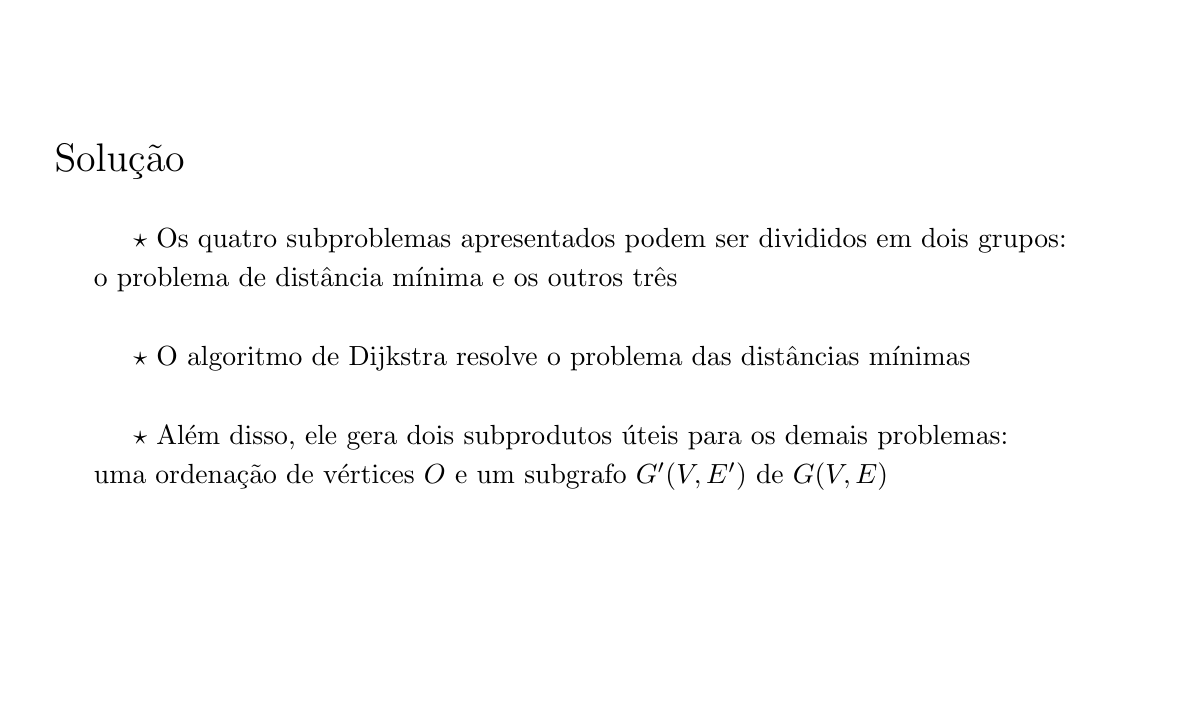
\begin{tikzpicture}
\node[draw,opacity=0] at (0, 0) {x};
\node[draw,opacity=0] at (14, 8) {x};

	\node[anchor=west] (title) at (0.0, 6.5) { \Large \bbbold{Solução} };

	\node[anchor=west] (a) at (1.0, 5.5) { $\star$ \bbtext{Os quatro subproblemas apresentados podem ser divididos em dois grupos:} };

	\node[anchor=west] (a1) at (0.5, 5.0) { \bbtext{o problema de distância mínima e os outros três} };


	\node[anchor=west] (b) at (1.0, 4.0) { $\star$ \bbtext{O algoritmo de Dijkstra resolve o problema das distâncias mínimas} };


	\node[anchor=west] (c) at (1.0, 3.0) { $\star$ \bbtext{Além disso, ele gera dois subprodutos úteis para os demais problemas:} };

	\node[anchor=west] (c1) at (0.5, 2.5) { \bbtext{uma ordenação de vértices $O$ e um subgrafo $G'(V, E')$ de $G(V, E)$} };


\end{tikzpicture}
\end{frame}
\begin{frame}[plain,t]
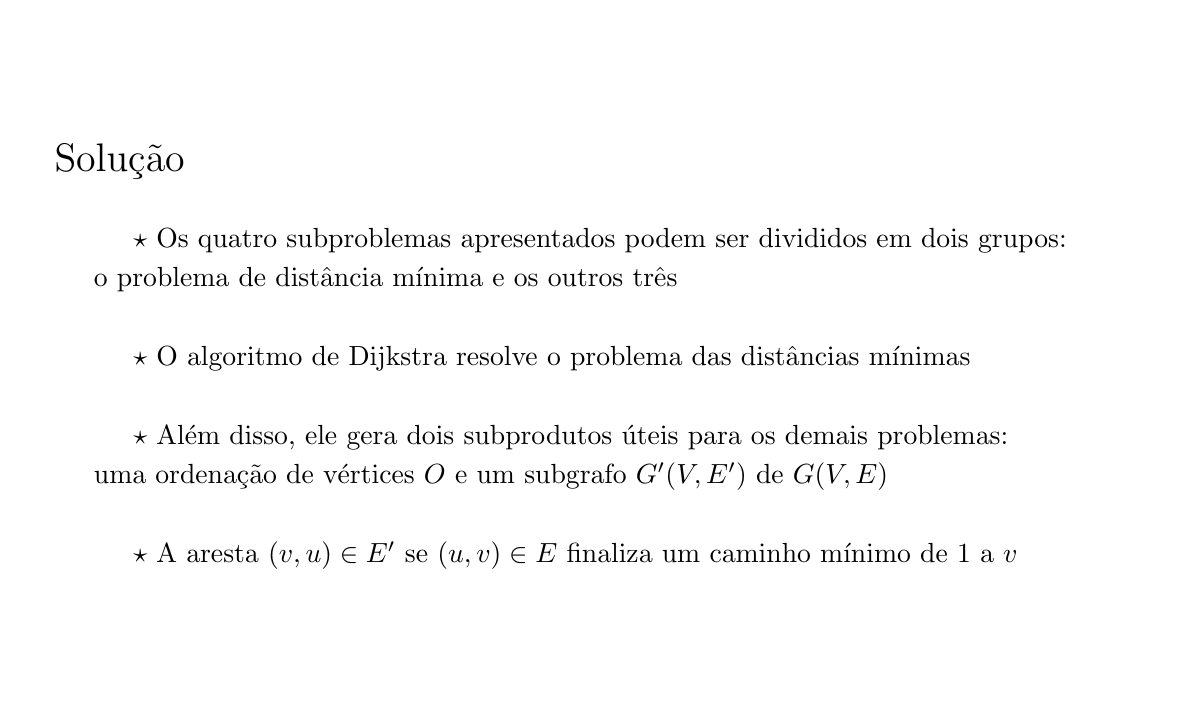
\begin{tikzpicture}
\node[draw,opacity=0] at (0, 0) {x};
\node[draw,opacity=0] at (14, 8) {x};

	\node[anchor=west] (title) at (0.0, 6.5) { \Large \bbbold{Solução} };

	\node[anchor=west] (a) at (1.0, 5.5) { $\star$ \bbtext{Os quatro subproblemas apresentados podem ser divididos em dois grupos:} };

	\node[anchor=west] (a1) at (0.5, 5.0) { \bbtext{o problema de distância mínima e os outros três} };


	\node[anchor=west] (b) at (1.0, 4.0) { $\star$ \bbtext{O algoritmo de Dijkstra resolve o problema das distâncias mínimas} };


	\node[anchor=west] (c) at (1.0, 3.0) { $\star$ \bbtext{Além disso, ele gera dois subprodutos úteis para os demais problemas:} };

	\node[anchor=west] (c1) at (0.5, 2.5) { \bbtext{uma ordenação de vértices $O$ e um subgrafo $G'(V, E')$ de $G(V, E)$} };



	\node[anchor=west] (d) at (1.0, 1.5) { $\star$ \bbtext{A aresta $(v, u)\in E'$ se $(u,v)\in E$ finaliza um  caminho mínimo de $1$ a $v$} };

\end{tikzpicture}
\end{frame}
\begin{frame}[plain,t]
\begin{tikzpicture}
\node[draw,opacity=0] at (0, 0) {x};
\node[draw,opacity=0] at (14, 8) {x};

	\node[anchor=west] (title) at (0.0, 7.5) { \Large \bbbold{Solução} };

	\node[anchor=west] (a) at (1.0, 6.5) { $\star$ \bbtext{A partir de $G'$ os três outros subproblemas podem ser resolvidos por DP} };

\end{tikzpicture}
\end{frame}
\begin{frame}[plain,t]
\begin{tikzpicture}
\node[draw,opacity=0] at (0, 0) {x};
\node[draw,opacity=0] at (14, 8) {x};

	\node[anchor=west] (title) at (0.0, 7.5) { \Large \bbbold{Solução} };

	\node[anchor=west] (a) at (1.0, 6.5) { $\star$ \bbtext{A partir de $G'$ os três outros subproblemas podem ser resolvidos por DP} };


	\node[anchor=west] (b) at (1.0, 5.5) { $\star$ \bbtext{Os casos base são: $\mathrm{minPaths}[1] = 1$ e $\mathrm{minEdges}[1] = \mathrm{maxEdges}[1] = 0$} };

\end{tikzpicture}
\end{frame}
\begin{frame}[plain,t]
\begin{tikzpicture}
\node[draw,opacity=0] at (0, 0) {x};
\node[draw,opacity=0] at (14, 8) {x};

	\node[anchor=west] (title) at (0.0, 7.5) { \Large \bbbold{Solução} };

	\node[anchor=west] (a) at (1.0, 6.5) { $\star$ \bbtext{A partir de $G'$ os três outros subproblemas podem ser resolvidos por DP} };


	\node[anchor=west] (b) at (1.0, 5.5) { $\star$ \bbtext{Os casos base são: $\mathrm{minPaths}[1] = 1$ e $\mathrm{minEdges}[1] = \mathrm{maxEdges}[1] = 0$} };


	\node[anchor=west] (c) at (1.0, 4.5) { $\star$ \bbtext{As transições são dadas por:} };

\end{tikzpicture}
\end{frame}
\begin{frame}[plain,t]
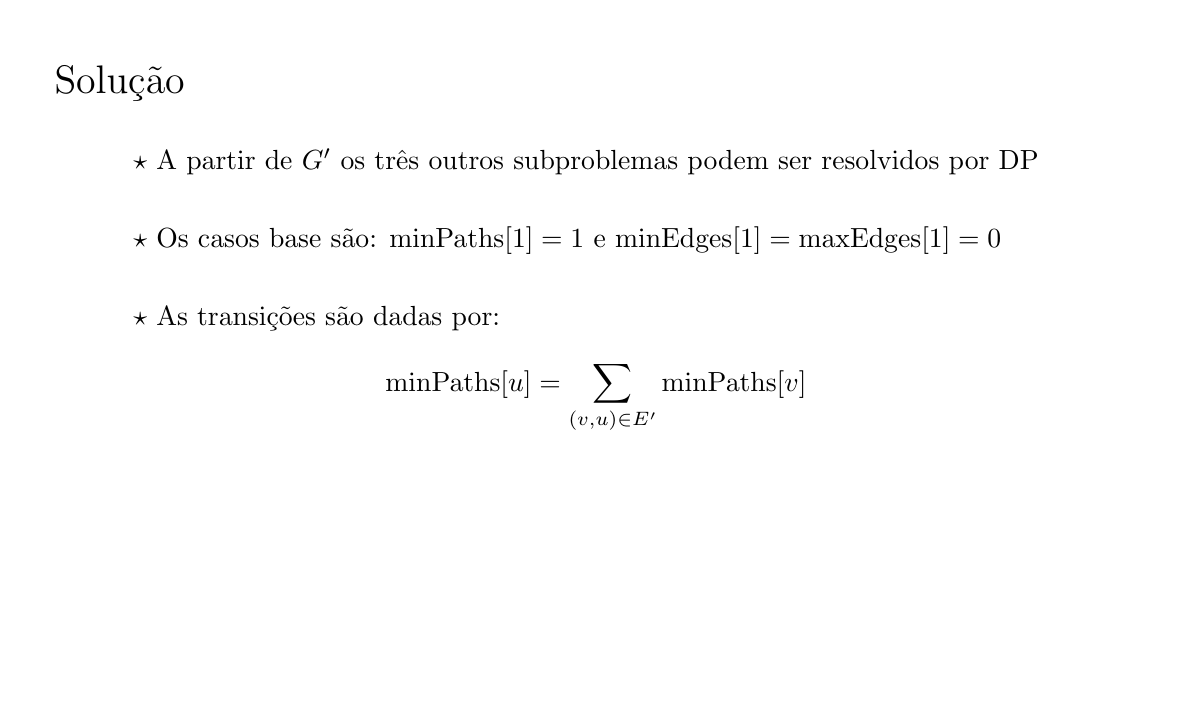
\begin{tikzpicture}
\node[draw,opacity=0] at (0, 0) {x};
\node[draw,opacity=0] at (14, 8) {x};

	\node[anchor=west] (title) at (0.0, 7.5) { \Large \bbbold{Solução} };

	\node[anchor=west] (a) at (1.0, 6.5) { $\star$ \bbtext{A partir de $G'$ os três outros subproblemas podem ser resolvidos por DP} };


	\node[anchor=west] (b) at (1.0, 5.5) { $\star$ \bbtext{Os casos base são: $\mathrm{minPaths}[1] = 1$ e $\mathrm{minEdges}[1] = \mathrm{maxEdges}[1] = 0$} };


	\node[anchor=west] (c) at (1.0, 4.5) { $\star$ \bbtext{As transições são dadas por:} };


	\node[] (d) at (7.0, 3.5) { $\displaystyle \mathrm{minPaths}[u] = \sum_{(v, u)\in E'} \mathrm{minPaths}[v]$ };

\end{tikzpicture}
\end{frame}
\begin{frame}[plain,t]
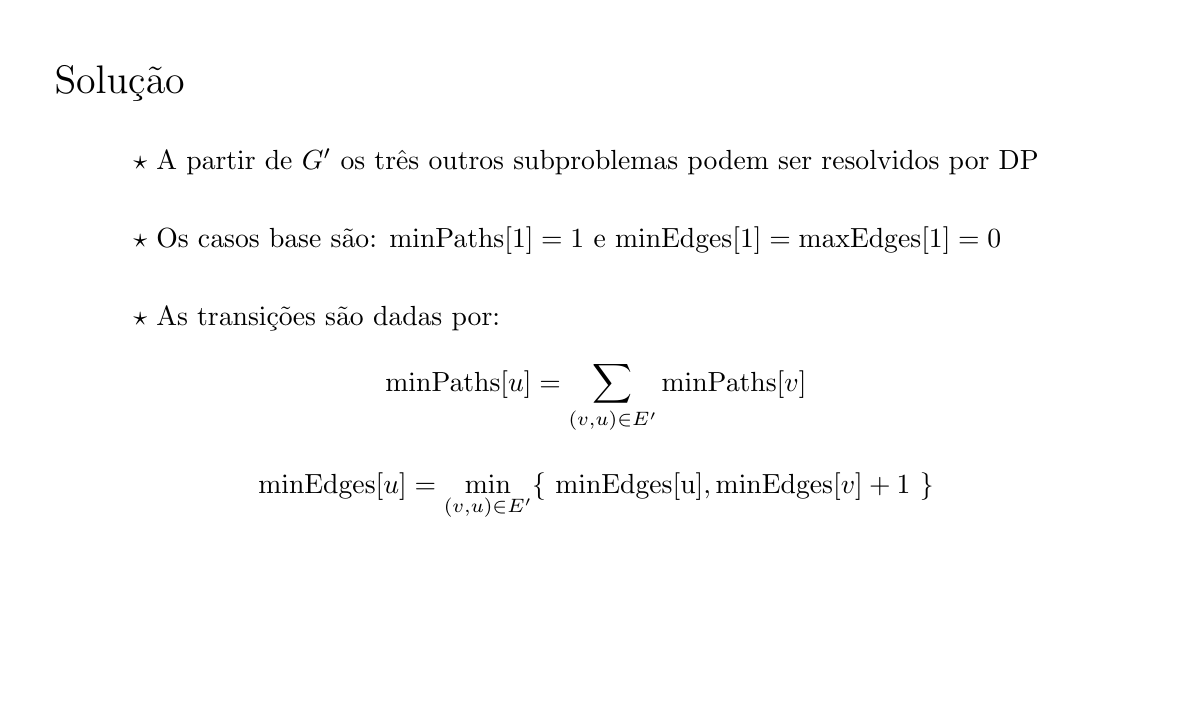
\begin{tikzpicture}
\node[draw,opacity=0] at (0, 0) {x};
\node[draw,opacity=0] at (14, 8) {x};

	\node[anchor=west] (title) at (0.0, 7.5) { \Large \bbbold{Solução} };

	\node[anchor=west] (a) at (1.0, 6.5) { $\star$ \bbtext{A partir de $G'$ os três outros subproblemas podem ser resolvidos por DP} };


	\node[anchor=west] (b) at (1.0, 5.5) { $\star$ \bbtext{Os casos base são: $\mathrm{minPaths}[1] = 1$ e $\mathrm{minEdges}[1] = \mathrm{maxEdges}[1] = 0$} };


	\node[anchor=west] (c) at (1.0, 4.5) { $\star$ \bbtext{As transições são dadas por:} };


	\node[] (d) at (7.0, 3.5) { $\displaystyle \mathrm{minPaths}[u] = \sum_{(v, u)\in E'} \mathrm{minPaths}[v]$ };


	\node[] (d1) at (7.0, 2.25) { $\displaystyle \mathrm{minEdges}[u] = \min_{(v, u)\in E'}\{\ \mathrm{minEdges[u]}, \mathrm{minEdges}[v] + 1 \ \}$ };

\end{tikzpicture}
\end{frame}
\begin{frame}[plain,t]
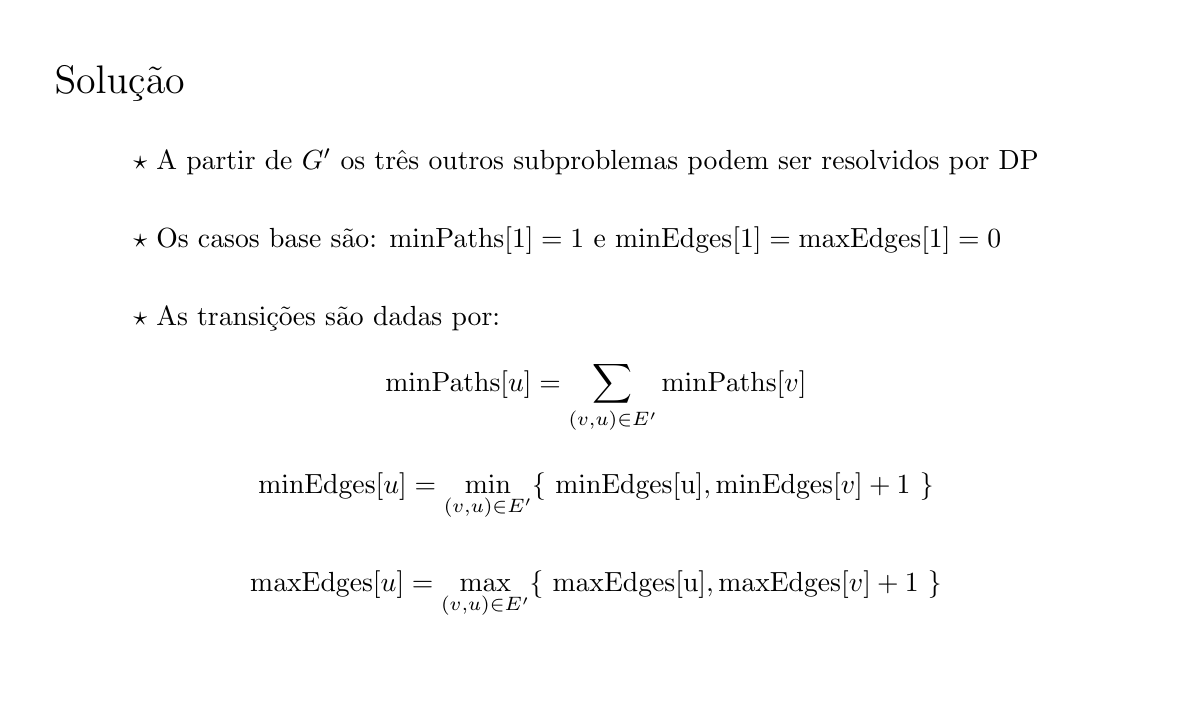
\begin{tikzpicture}
\node[draw,opacity=0] at (0, 0) {x};
\node[draw,opacity=0] at (14, 8) {x};

	\node[anchor=west] (title) at (0.0, 7.5) { \Large \bbbold{Solução} };

	\node[anchor=west] (a) at (1.0, 6.5) { $\star$ \bbtext{A partir de $G'$ os três outros subproblemas podem ser resolvidos por DP} };


	\node[anchor=west] (b) at (1.0, 5.5) { $\star$ \bbtext{Os casos base são: $\mathrm{minPaths}[1] = 1$ e $\mathrm{minEdges}[1] = \mathrm{maxEdges}[1] = 0$} };


	\node[anchor=west] (c) at (1.0, 4.5) { $\star$ \bbtext{As transições são dadas por:} };


	\node[] (d) at (7.0, 3.5) { $\displaystyle \mathrm{minPaths}[u] = \sum_{(v, u)\in E'} \mathrm{minPaths}[v]$ };


	\node[] (d1) at (7.0, 2.25) { $\displaystyle \mathrm{minEdges}[u] = \min_{(v, u)\in E'}\{\ \mathrm{minEdges[u]}, \mathrm{minEdges}[v] + 1 \ \}$ };


	\node[] (d2) at (7.0, 1.0) { $\displaystyle \mathrm{maxEdges}[u] = \max_{(v, u)\in E'}\{\ \mathrm{maxEdges[u]}, \mathrm{maxEdges}[v] + 1 \ \}$ };

\end{tikzpicture}
\end{frame}
\begin{frame}[plain,t]

\inputsnippet{cpp}{73}{79}{codes/1202.cpp}

\end{frame}
\begin{frame}[plain,t]

\inputsnippet{cpp}{14}{33}{codes/1202.cpp}

\end{frame}
\begin{frame}[plain,t]

\inputsnippet{cpp}{35}{51}{codes/1202.cpp}

\end{frame}
\begin{frame}[plain,t]

\inputsnippet{cpp}{53}{70}{codes/1202.cpp}

\end{frame}
\end{document}
